\documentclass[conference]{IEEEtran}
\IEEEoverridecommandlockouts
\usepackage{cite}
\usepackage{amsmath,amssymb}
\usepackage{graphicx}
\usepackage{booktabs}
\usepackage{multirow}
\usepackage{url}
\usepackage{xcolor}
\usepackage{tikz}
\usetikzlibrary{arrows.meta,positioning}
\usepackage{pgfplots}
\pgfplotsset{compat=1.17}

\newcommand{\sig}[1]{\textbf{#1}}

\begin{document}

\title{Structure-Aware, Fully Local Retrieval-Augmented Generation for Indian Statutory Law}

\author{\IEEEauthorblockN{Author Name}
\IEEEauthorblockA{\textit{Department} \\
\textit{Institution}\\
City, Country \\
email@example.com}
}

\maketitle

\begin{abstract}
We present a retrieval-augmented generation (RAG) system for Indian statutory law that runs entirely on a consumer
laptop (one 8\,GB GPU) with open models. Built in three stages and evaluated as an ablation on the IndiaStatRAG
span-retrieval benchmark, the final system reaches 0.757 macro evidence recall at an 8,000-character budget on the
352-question test set, against 0.242 for the strongest BM25 baseline, and beats it in all six answerable
categories. Most of the gain comes from statute-aligned retrieval units, dense retrieval and a cross-encoder. Of
five ways to use a local 8B language model, only cited answer generation helped significantly: +0.176 fact coverage
over an extractive baseline, with no citation to a provision outside the retrieved evidence. A provision-level
cross-reference graph, applied only to two-part questions, raises the share of cross-reference questions with all
required provisions retrieved from 0.314 to 0.490 ($p=0.002$) without changing any other category. Deterministic
abstention rules reject 77\% of unanswerable test questions at 3.2\% false abstention; every miss was a foreign-law
or case-law question. With gold evidence in context, the same 8B generator covers 90\% of required facts,
identifying retrieval as the main bottleneck. All tuning used a development subset, and each frozen system was run
once on the test set.
\end{abstract}

\begin{IEEEkeywords}
retrieval-augmented generation, legal information retrieval, Indian law, dense retrieval, abstention, local language models
\end{IEEEkeywords}

\section{Introduction}

Legal question answering is a high-stakes use of large language models (LLMs): commercial legal research tools
built on retrieval-augmented generation still hallucinate and mis-cite authority~\cite{magesh2024hallucination}.
Indian statutory law adds specific difficulties. The corpus spans Central law and more than thirty States and
Union Territories, with near-duplicate Acts, amendment Acts, Rules and Regulations. Questions often paraphrase an
Act's name or describe a situation without naming any law, an answer may require two provisions that cite each
other, and the correct provision for one State can be wrong for another.

This paper asks how far a system can go when everything must run locally, on one laptop GPU, with open models
and no paid APIs. We study five research questions: whether structure-aligned retrieval units improve recall and
precision at fixed budgets (RQ1); whether a small local LLM used for query understanding closes the gap on
situational questions (RQ2); whether Act routing and cross-reference expansion help multi-provision and
jurisdictional questions (RQ3); whether calibrated abstention can reject unanswerable questions without
unacceptable false abstention (RQ4); and how faithful locally generated, cited answers are (RQ5).

Our contributions are: (1) a structure-aware hybrid retrieval pipeline over a 15,325-document Indian statute
corpus, with a budget-aware packer and deterministic abstention; (2) a controlled ablation of five uses of a local
8B LLM, showing that at this scale only answer generation helps; (3) a provision-level cross-reference graph with
question-shape gating that significantly improves multi-provision retrieval; and (4) an evaluation protocol
designed against overfitting, with a pre-registered holdout and a single frozen test run.

\section{Related Work}

\textbf{Retrieval-augmented generation.} RAG conditions generation on retrieved passages~\cite{lewis2020rag}.
Lexical retrieval with BM25~\cite{robertson2009bm25} remains a strong baseline; dense bi-encoders~\cite{karpukhin2020dpr}
and recent multilingual embedding models~\cite{chen2024bgem3,wang2024e5,zhang2025qwen3emb} improve semantic
matching, and cross-encoders rerank candidates~\cite{nogueira2019bert}. Reciprocal rank fusion (RRF) combines
ranked lists without score calibration~\cite{cormack2009rrf}.

\textbf{LLMs inside retrieval.} HyDE generates a hypothetical document and retrieves with its
embedding~\cite{gao2023hyde}. LLMs can rerank passages, and listwise prompting, where the model sees several
candidates together, is effective with large models~\cite{sun2023rankgpt}. Tool-using agents interleave reasoning
and retrieval actions~\cite{yao2023react}. We test these ideas with an 8B model under a strict compute budget.

\textbf{Indian legal NLP.} Prior work covers domain pre-training (InLegalBERT~\cite{paul2023inlegalbert}), case-law
understanding benchmarks (IL-TUR~\cite{joshi2024iltur}) and statute and precedent retrieval
(AILA~\cite{bhattacharya2019aila}). These target different tasks and metrics; we evaluate on IndiaStatRAG, which
scores character-level evidence spans and cited answers over statutes~\cite{indiastatrag}. No other system has
been evaluated on it, so all comparisons here are to baselines run on the same official scorer.

\section{Task and Data}

\textbf{Benchmark.} IndiaStatRAG~\cite{indiastatrag} has 502 verified questions in seven categories
(Table~\ref{tab:bench}). A system returns ranked character spans at budgets of 2,000, 8,000 (headline) and 32,000
characters. A gold location counts as found when the returned spans cover at least $\tau=0.5$ of it (0.8 and 1.0
are also reported); gold evidence comes in groups of interchangeable locations, so any copy of the same Act
counts. The scorer reports evidence recall, evidence precision, all-groups (every required group found), document
recall and MRR. Abstention means returning nothing at the 8,000 budget. Optional answers are scored for fact
coverage, citation recall and precision on (document, provision key), and grounding of quotes of 12 or more
characters.

\begin{table}[t]
\caption{IndiaStatRAG categories and split sizes}
\label{tab:bench}
\centering
\footnotesize
\begin{tabular}{@{}lrrl@{}}
\toprule
Category & Dev & Test & What it tests \\
\midrule
situational & 40 & 93 & fact pattern; Act never named \\
provision\_lookup & 23 & 53 & named Act and provision \\
cross\_reference & 21 & 51 & two provisions, both required \\
jurisdictional & 21 & 50 & one State's version of a law \\
numeric\_threshold & 15 & 36 & penalties, limits, periods \\
definitional & 15 & 34 & definitions clauses \\
unanswerable & 15 & 35 & correct output is empty \\
\bottomrule
\end{tabular}
\end{table}

\textbf{Corpus.} 15,325 documents: 8,797 State Acts, 839 Central Acts, 4,438 Rules and 1,251 Regulations, each with
canonical text, metadata (titles, jurisdiction, year, parent Act) and a structure file listing provisions with
character offsets. Gold spans are short (median 751 characters, 90th percentile 2,642).

\section{System}

The system was built in three stages (Fig.~\ref{fig:arch}). Plan~A is retrieval without an LLM, Plan~B adds a local
LLM, and Plan~C adds Act-level and cross-reference structure.

\begin{figure}[t]
\centering
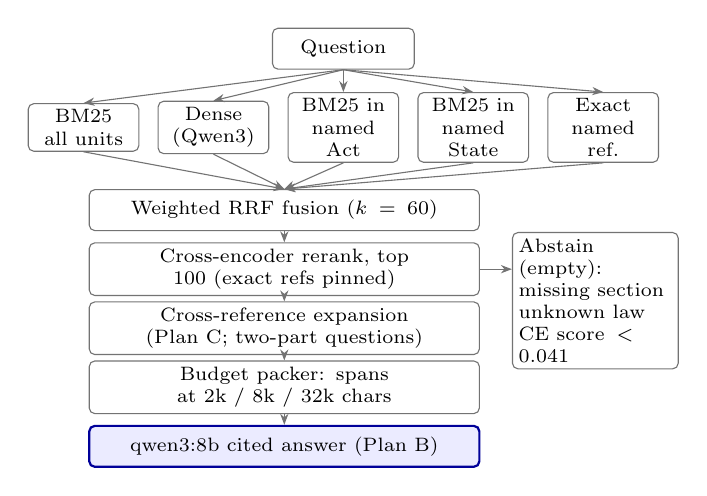
\begin{tikzpicture}[font=\scriptsize,
  box/.style={draw=black!55, rounded corners=2pt, align=center, inner sep=2.2pt, minimum height=5.2mm},
  arr/.style={-{Stealth[length=1.4mm]}, black!55}]
\node[box, minimum width=18mm] (q) at (0,0) {Question};
\node[box, text width=12.5mm] (s0) at (-3.3,-1.0) {BM25\\all units};
\node[box, text width=12.5mm] (s1) at (-1.65,-1.0) {Dense\\(Qwen3)};
\node[box, text width=12.5mm] (s2) at (0,-1.0) {BM25 in\\named Act};
\node[box, text width=12.5mm] (s3) at (1.65,-1.0) {BM25 in\\named State};
\node[box, text width=12.5mm] (s4) at (3.3,-1.0) {Exact\\named ref.};
\foreach \i in {0,...,4} { \draw[arr] (q.south) -- (s\i.north); }
\node[box, text width=48mm] (f) at (-0.75,-2.05) {Weighted RRF fusion ($k=60$)};
\foreach \i in {0,...,4} { \draw[arr] (s\i.south) -- (f.north); }
\node[box, text width=48mm] (r) at (-0.75,-2.8) {Cross-encoder rerank, top 100 (exact refs pinned)};
\node[box, text width=48mm] (x) at (-0.75,-3.55) {Cross-reference expansion (Plan C; two-part questions)};
\node[box, text width=48mm] (p) at (-0.75,-4.3) {Budget packer: spans at 2k / 8k / 32k chars};
\node[box, text width=48mm, fill=blue!8, draw=blue!60!black, thick] (a) at (-0.75,-5.05) {qwen3:8b cited answer (Plan B)};
\node[box, text width=19.5mm, align=left] (ab) at (3.2,-3.2) {Abstain (empty):\\missing section\\unknown law\\CE score${}<0.041$};
\draw[arr] (f) -- (r); \draw[arr] (r) -- (x); \draw[arr] (x) -- (p); \draw[arr] (p) -- (a);
\draw[arr] (r.east) -- (ab.west |- r.east);
\end{tikzpicture}
\caption{The final system. Three of the five retrieval signals come from rule-based query parsing; the LLM is used
only to write the cited answer.}
\label{fig:arch}
\end{figure}

\subsection{Plan A: Structure-Aware Hybrid Retrieval}

\textbf{Retrieval units.} Every document is cut into 884,128 units: 363,539 provisions from the structure files,
262,658 sub-units (long provisions split along sub-sections into pieces of at most 2,000 characters) and 257,931
gap windows of 1,200 characters over text no provision covers, so the whole corpus is searchable. Units with
identical normalised text form duplicate classes; 783,706 representatives are indexed. On dev, all 205 gold
locations coincide exactly with one provision unit.

\textbf{Signals.} (i) BM25 over title, label and unit text; (ii) dense retrieval with Qwen3-Embedding-0.6B
\cite{zhang2025qwen3emb}, exact fp16 cosine search on the GPU, chosen on a dev-only proxy where it tied
e5-large-instruct~\cite{wang2024e5} at recall@10 0.907 and led on situational questions, ahead of
bge-m3~\cite{chen2024bgem3} (0.867) and InLegalBERT~\cite{paul2023inlegalbert} (0.218); (iii) rule-based query
parsing, which matches Act titles against the corpus's own titles and extracts section numbers and State names,
yielding BM25 restricted to the named Act, BM25 restricted to the named State, and the exact named provision.
Lists are fused with weighted RRF~\cite{cormack2009rrf} and the top 100 are reranked by the bge-reranker-v2-m3
cross-encoder; exact named provisions stay pinned on top.

\textbf{Budget packer.} The packer walks the ranking, emits one unit per duplicate class, skips already-returned
text, and for a long provision that no longer fits emits the best window inside it, centred on its best-ranked
sub-unit.

\textbf{Abstention.} The system abstains when (1) the question names a resolvable Act and a section number that
exists in no copy of it, (2) it names a law matching no corpus title, or (3) the top cross-encoder score is below
0.041, a threshold set on dev with a rule fixed in advance (maximise abstention minus twice the false-abstention
rate, subject to false abstention at most 5\%).

\subsection{Plan B: A Local LLM Layer}

We use qwen3:8b~\cite{yang2025qwen3} (4-bit, thinking off, temperature 0) through Ollama~\cite{ollama} with
JSON-schema-constrained output. The model needs 6.5\,GB of VRAM at an 8k-token context, so the runner executes in
stages (LLM, then GPU retrieval with the LLM unloaded, then LLM), and every LLM call is cached by model digest,
prompt version and input. We tested five uses: query analysis (named and candidate Acts, keywords, jurisdiction)
feeding Act-restricted retrieval lists; HyDE~\cite{gao2023hyde}; pointwise LLM reranking of the top 20 (yes/no
log-probability mixed with the cross-encoder score); an LLM abstention judge; and cited answer generation. The
answer prompt receives the top eight packed provisions, numbered, and must answer in 1--3 sentences in their own
words, quote the decisive phrase, and cite provisions by number or abstain. Post-processing keeps quotation marks
only around text verified, under the scorer's normalisation, against the cited provisions.

\subsection{Plan C: Act Routing and Cross-Reference Expansion}

\textbf{Act routing.} A card per document (titles, type, jurisdiction, parent Act, section headings) is indexed with
BM25 and dense embeddings; retrieval is then repeated inside the top five routed Acts.

\textbf{Cross-reference graph.} For each provision, citations in its text (``section 7'', ``sections 10 to 12'',
``rule 3'', ``section 8 of the Act'') are resolved to provisions of the same document, or of the parent Act for
Rules and Regulations; citations of other named Acts are skipped. This yields 184,299 edges. The graph contains
the gold link for 13 of 14 dev cross-reference questions used for design.

\textbf{Gated expansion.} Inserting cited provisions after the top-ranked units helps cross-reference questions
but pushes correct evidence out of the budget elsewhere. Reranking the partners with the cross-encoder fails
because a partner answers only the \emph{second part} of a compound question. We therefore expand only questions
that split into two or more parts (11 of 14 cross-reference questions versus 6 of 76 others on dev), score each
cited or citing provision of the top three units against each part separately, and insert at most two per unit
whose best part score reaches the existing 0.041 threshold.

\section{Evaluation Protocol}

The benchmark's split gives 150 dev and 352 test questions. We split dev, stratified by category, into dev\_tune
(100) for all design and selection and dev\_holdout (50), scored only for frozen configurations with a logged
note. A component was adopted only if it gave a significant paired gain on dev\_tune without regressions elsewhere;
the single exception (Plan~C's expansion) was adopted by explicit decision with its non-significance recorded, and
its holdout pass criterion was committed to version control before the holdout run. The test split was opened
once: each frozen system ran from a tagged commit, a driver refused to run on a modified tree, and every
evaluation was logged. Differences are paired bootstrap estimates~\cite{efron1993bootstrap} with 95\% confidence
intervals. An overfitting audit of Plan~A found out-of-fold abstention of 0.937 against 1.000 in-sample, 99\%
abstention on synthetic questions about fake sections of 600 unseen Acts with 0\% false abstention, and flat
sensitivity (0.765--0.792 macro recall across 16 perturbed settings, frozen 0.769).

\section{Results}

Table~\ref{tab:main} summarises the single test run. B-full shares Plan~A's retrieval and is omitted from the
retrieval rows. Fig.~\ref{fig:cats} shows recall per category.

\begin{table}[t]
\caption{Test results (macro over six answerable categories)}
\label{tab:main}
\centering
\footnotesize
\setlength{\tabcolsep}{3pt}
\begin{tabular}{@{}lccccccc@{}}
\toprule
System & R@2k & R@8k & R@32k & P@8k & MRR & XR-all & Abst./FA \\
\midrule
BM25 two-stage & .106 & .242 & .349 & .033 & .133 & .098 & .00/.00 \\
BM25 windows & .143 & .283 & .368 & .034 & .172 & .118 & .00/.00 \\
Dense only & .476 & .649 & .807 & .101 & .464 & .333 & .00/.00 \\
Plan A & .592 & .747 & .835 & .122 & .604 & .314 & .77/.03 \\
Plan C (final) & \sig{.601} & \sig{.757} & \sig{.844} & .119 & \sig{.608} & \sig{.490} & .77/.03 \\
\bottomrule
\end{tabular}
\\[2pt]
\raggedright\scriptsize R@B: evidence recall at budget $B$; P: precision; XR-all: cross-reference questions with
all required groups found; Abst./FA: abstention on unanswerable / false abstention on answerable questions.
\end{table}

\begin{figure}[t]
\centering
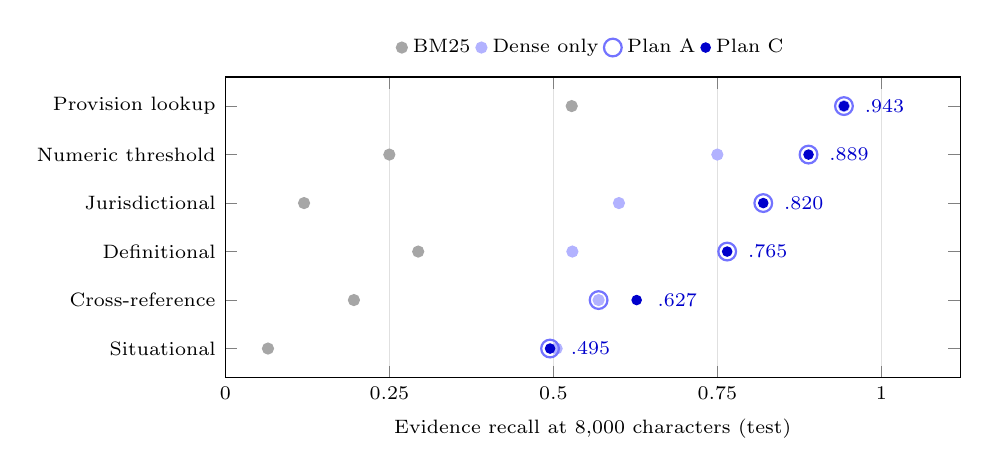
\begin{tikzpicture}
\begin{axis}[width=0.9\columnwidth, height=5.4cm, xmin=0, xmax=1.12, xtick={0,0.25,0.5,0.75,1},
  symbolic y coords={Situational,Cross-reference,Definitional,Jurisdictional,Numeric threshold,Provision lookup},
  ytick=data, enlarge y limits=0.12, xmajorgrids, grid style={black!12},
  tick label style={font=\scriptsize}, label style={font=\scriptsize},
  xlabel={Evidence recall at 8,000 characters (test)},
  legend style={font=\scriptsize, at={(0.5,1.03)}, anchor=south, legend columns=4, draw=none}]
\addplot[only marks, mark=*, mark size=2pt, black!35] coordinates {(0.528,Provision lookup) (0.25,Numeric threshold) (0.12,Jurisdictional) (0.294,Definitional) (0.196,Cross-reference) (0.065,Situational)};
\addlegendentry{BM25}
\addplot[only marks, mark=*, mark size=2pt, blue!30] coordinates {(0.943,Provision lookup) (0.75,Numeric threshold) (0.6,Jurisdictional) (0.529,Definitional) (0.569,Cross-reference) (0.505,Situational)};
\addlegendentry{Dense only}
\addplot[only marks, mark=o, mark size=3.2pt, blue!55, thick] coordinates {(0.943,Provision lookup) (0.889,Numeric threshold) (0.82,Jurisdictional) (0.765,Definitional) (0.569,Cross-reference) (0.495,Situational)};
\addlegendentry{Plan A}
\addplot[only marks, mark=*, mark size=1.7pt, blue!80!black, nodes near coords, point meta=explicit symbolic,
  every node near coord/.style={anchor=west, font=\scriptsize, xshift=4pt}] coordinates {(0.943,Provision lookup) [.943] (0.889,Numeric threshold) [.889] (0.82,Jurisdictional) [.820] (0.765,Definitional) [.765] (0.627,Cross-reference) [.627] (0.495,Situational) [.495]};
\addlegendentry{Plan C}
\end{axis}
\end{tikzpicture}
\caption{Test recall per category. Dense retrieval gives most of the gain over BM25; Plan A adds definitional,
jurisdictional and numeric questions; Plan C adds cross-reference. Situational remains weakest.}
\label{fig:cats}
\end{figure}

\textbf{Retrieval.} Table~\ref{tab:paired} gives paired differences. The final system beats the strongest BM25
baseline in every category (all differences significant), with the largest gains on jurisdictional (+0.700) and
numeric (+0.639) questions. Plan~A improves on dense-only retrieval by +0.073 overall, significantly on
definitional and jurisdictional questions; it is not better on situational questions. Plan~C changes no question
outside cross-reference at any budget and raises cross-reference all-groups from 0.314 to 0.490 (+0.176, 95\% CI
[+0.059, +0.294], $p=0.002$; 10 questions better, 1 worse). Results barely move at $\tau=1.0$ (e.g.\
cross-reference 0.618, jurisdictional 0.820), because provision-aligned units return whole provisions.

\begin{table}[t]
\caption{Paired differences in test recall at 8,000 characters}
\label{tab:paired}
\centering
\footnotesize
\setlength{\tabcolsep}{2.6pt}
\begin{tabular}{@{}lccccccc@{}}
\toprule
Comparison & XR & DEF & JUR & NUM & PROV & SIT & All \\
\midrule
Plan C $-$ BM25 & \sig{+.431} & \sig{+.471} & \sig{+.700} & \sig{+.639} & \sig{+.415} & \sig{+.430} & \sig{+.498} \\
Plan A $-$ Dense & .000 & \sig{+.235} & \sig{+.220} & +.139 & .000 & $-$.011 & \sig{+.073} \\
Plan C $-$ Plan A & +.059 & .000 & .000 & .000 & .000 & .000 & +.009 \\
\bottomrule
\end{tabular}
\\[2pt]
\raggedright\scriptsize Bold: paired bootstrap 95\% CI excludes 0. ``All'': 317 answerable questions; overall CIs
[+.442, +.555], [+.024, +.123] and [$-$.003, +.022].
\end{table}

\textbf{Pre-registered criteria.} The final system meets all minimum criteria fixed before the test run: it beats
the best BM25 baseline in every answerable category, significantly on situational, jurisdictional and
cross-reference questions, and abstains on 77.1\% of unanswerable questions at 3.2\% false abstention. The stretch
goal of an order-of-magnitude precision gain was not reached (3.6$\times$).

\textbf{Answers.} Table~\ref{tab:answers} reports answer quality. LLM answers improve fact coverage by +0.176 and
citation recall by +0.114 over an extractive baseline that quotes the top provision. Of 904 citations written by
the LLM systems, none refers to a non-existent provision or to a document outside the retrieved context. All
scored quotes were grounded, but only 40 of 317 answers carried a scored quote, because the model tends to quote
with single quotation marks, which the scorer ignores.

\begin{table}[t]
\caption{Answer quality on test (317 answerable questions)}
\label{tab:answers}
\centering
\footnotesize
\begin{tabular}{@{}lccc@{}}
\toprule
System & Fact cov. & Cit. recall & Cit. precision \\
\midrule
Extractive (top provision) & .534 & .535 & .580 \\
Plan B (qwen3:8b) & .709 & .648 & .591 \\
Plan C (final) & \sig{.722} & \sig{.655} & \sig{.597} \\
\midrule
Plan B $-$ extractive & \sig{+.176} & \sig{+.114} & +.011 \\
Plan C $-$ Plan B & \sig{+.013} & +.006 & +.006 \\
\bottomrule
\end{tabular}
\end{table}

\section{Analysis}

\subsection{What the Local LLM Did Not Do}

On dev\_tune, none of the retrieval-side LLM stages produced a significant gain (Table~\ref{tab:planb}). Query
analysis failed on legal knowledge rather than formatting: the Acts the model named included the gold Act for only
about 30\% of situational questions and for no definitional question, and its extra lists diluted the reranker's
candidate pool (the fused top 100 held 0.90 of gold groups, against 0.95 in the dense list alone). The pointwise reranker added three questions at
about 45\,s per question. The abstention judge rated every answerable question at $P(\text{answerable})\ge0.94$
and never fired. For answers, a few-shot prompt reduced citation recall ($-0.122$, significant), thinking mode
added $+0.022$ (not significant) at five times the latency, and llama3.1:8b~\cite{dubey2024llama3} was
significantly worse on all three answer metrics. The answer to RQ2 is therefore negative at this model size.

\begin{table}[t]
\caption{Plan B retrieval ablation on dev\_tune (recall at 8k)}
\label{tab:planb}
\centering
\footnotesize
\setlength{\tabcolsep}{3.5pt}
\begin{tabular}{@{}lccccr@{}}
\toprule
Configuration & XR & JUR & SIT & FA & LLM s/q \\
\midrule
Plan A & .500 & .786 & .852 & .011 & -- \\
+ LLM query analysis & .500 & .714 & .852 & .033 & 5 \\
+ HyDE & .500 & .786 & .852 & .022 & 10 \\
+ pointwise LLM rerank & .571 & .857 & .889 & .022 & 55 \\
+ LLM abstention judge & .571 & .857 & .889 & .022 & 58 \\
\bottomrule
\end{tabular}
\\[2pt]
\raggedright\scriptsize Definitional, numeric and provision-lookup recall are unchanged (.700, .900, 1.000). No
difference is significant.
\end{table}

\subsection{Act Routing}

Card-based dense routing ranked the gold Act better than Plan~A's own document ranking on jurisdictional and
definitional questions, but adding retrieval inside the top five routed Acts changed nothing overall: Plan~A
already placed the gold Act among its top five documents for 91\% of dev\_tune questions. Routing was not adopted.

\subsection{Error Analysis}

Fig.~\ref{fig:errors} classifies the 368 gold evidence groups of the test set. The largest failure is the right Act
never reaching the context (48 groups), concentrated in situational questions; no group failed because another
State's copy of a provision was returned. All eight missed abstentions are foreign law (UK Companies Act 2006,
the constitutions of Nepal and South Africa, a UAE labour decree, Magna Carta) or case law (three judgments). Dev's
unanswerable questions were dominated by real Acts with non-existent sections, which the rules catch (16 of 16 on
test). Situational recall fell from 0.750 on dev to 0.495 on test, but untuned dense-only retrieval fell
identically (0.750 to 0.505), suggesting a harder test subset rather than overfitting.

\begin{figure}[t]
\centering
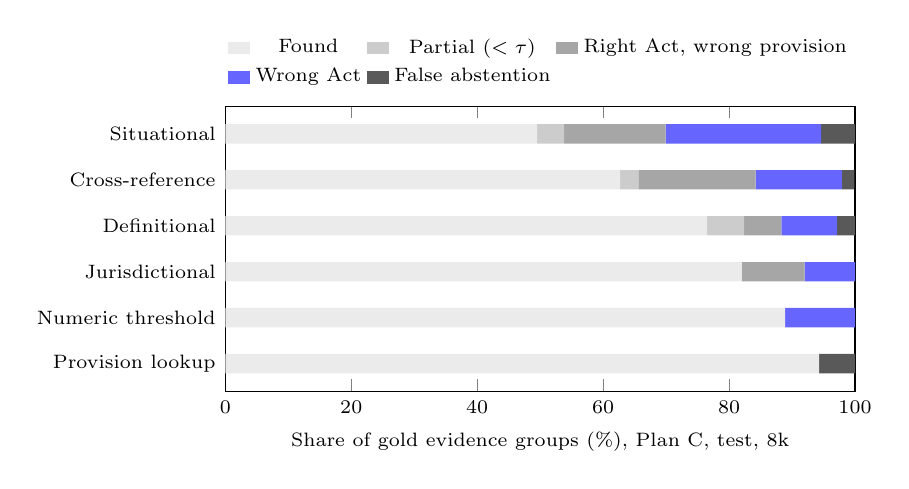
\begin{tikzpicture}
\begin{axis}[xbar stacked, width=0.79\columnwidth, height=5.2cm, xmin=0, xmax=100, bar width=7pt,
  legend image code/.code={\fill[#1] (0cm,-0.08cm) rectangle (0.28cm,0.08cm);},
  symbolic y coords={Provision lookup,Numeric threshold,Jurisdictional,Definitional,Cross-reference,Situational},
  ytick=data, enlarge y limits=0.12, tick label style={font=\scriptsize}, label style={font=\scriptsize},
  xlabel={Share of gold evidence groups (\%), Plan C, test, 8k},
  legend style={font=\scriptsize, at={(0.5,1.03)}, anchor=south, legend columns=3, draw=none}]
\addplot[fill=black!8, draw=none] coordinates {(94.3,Provision lookup) (88.9,Numeric threshold) (82.0,Jurisdictional) (76.5,Definitional) (62.7,Cross-reference) (49.5,Situational)};
\addlegendentry{Found}
\addplot[fill=black!20, draw=none] coordinates {(0,Provision lookup) (0,Numeric threshold) (0,Jurisdictional) (5.9,Definitional) (2.9,Cross-reference) (4.3,Situational)};
\addlegendentry{Partial ($<\tau$)}
\addplot[fill=black!35, draw=none] coordinates {(0,Provision lookup) (0,Numeric threshold) (10.0,Jurisdictional) (5.9,Definitional) (18.6,Cross-reference) (16.1,Situational)};
\addlegendentry{Right Act, wrong provision}
\addplot[fill=blue!60, draw=none] coordinates {(0,Provision lookup) (11.1,Numeric threshold) (8.0,Jurisdictional) (8.8,Definitional) (13.7,Cross-reference) (24.7,Situational)};
\addlegendentry{Wrong Act}
\addplot[fill=black!65, draw=none] coordinates {(5.7,Provision lookup) (0,Numeric threshold) (0,Jurisdictional) (2.9,Definitional) (2.0,Cross-reference) (5.4,Situational)};
\addlegendentry{False abstention}
\end{axis}
\end{tikzpicture}
\caption{Outcome per gold evidence group on test. Retrieving the wrong Act is the largest failure, mostly on
situational questions.}
\label{fig:errors}
\end{figure}

\subsection{Upper Bounds and Post-Test Exploration}

\textbf{Oracle context (dev\_tune).} Given the gold provisions instead of retrieved ones, the same answer stage
reaches 0.900 fact coverage, 0.967 citation recall and 0.989 citation precision (vs.\ 0.739, 0.789, 0.685), so
retrieval is the main bottleneck for answer quality (RQ5).

\textbf{Agent (dev only).} A qwen3:8b agent with search, table-of-contents and read tools (at most six steps),
started from Plan~C's results, improved pooled dev recall at 8k by +0.052 [+0.019, +0.093] but lowered citation
recall significantly, and its large dev\_tune gains at small budgets did not replicate on dev\_holdout. Its reads
came almost entirely from Plan~C's top eight provisions: the gain came from \emph{listwise} choice among
candidates, consistent with~\cite{sun2023rankgpt}, whereas pointwise reranking had failed.

\textbf{Listwise selection (post-test).} Turning that behaviour into a fixed stage (the LLM picks at most two of
the top eight provisions from one-line snippets) passed a pre-registered dev gate (+0.048 [+0.004, +0.093]) and
was then run once on test, labelled as post-test: recall at 8k +0.024 (not significant), recall at 2k +0.052 and
MRR +0.057 (both significant). It ranks better but adds little at the headline budget, and because it was designed
after the test set was spent it is reported as evidence for future work, not as a revised result.

\section{Limitations}

The benchmark's questions and labels were drafted and verified by LLMs rather than legal experts. No external
system has been evaluated on it, so comparisons are to baselines on the same scorer. Per-category samples are
small (15--40 dev and 34--93 test questions). The abstention rules and query parser were written after reading
dev questions; they generalised to unseen Acts but not to foreign and case law. The embedder was chosen on a
dev-derived proxy. Only models of at most 8B parameters at 4-bit fit the hardware alongside retrieval. Quote
grounding was measured on few answers.

\section{Conclusion}

A fully local RAG system on one laptop GPU retrieves Indian statutory evidence about three times better than
BM25 and writes cited answers that never cite outside their evidence. The gains come from statute structure and
strong open retrieval models; asking a small LLM what the law is did not help, while letting it write the answer
and, post hoc, choose among candidates did. The largest remaining failures---identifying the governing Act for a
described situation and recognising out-of-scope foreign or case law---define the next steps, together with
expert validation of the benchmark and a fresh test set.

\bibliographystyle{IEEEtran}
\bibliography{refs}

\end{document}
